\subsection{Prompt Curation} \label{sec:prompt} 

To endow the \model with comprehensive spatio-temporal reasoning capabilities, we synthesized a high-fidelity instruction dataset grounded in large-scale, real-world user behaviors. This dataset spans the full spectrum of user needs, covering atomic queries such as POI retrieval as well as composite, multi-constraint tasks like intricate itinerary planning.

We leveraged anonymized online user logs spanning a three-month window as our primary data source, with a volume of 30 million. The critical challenge lies in distilling these noisy, unstructured interactions into a structured, high-diversity instruction dataset suitable for training a sophisticated agent. To achieve this, we constructed a hierarchical \textbf{Intent Taxonomy}. This taxonomy functions as a rigorous framework for precise annotation, quantitative distribution analysis, and controlled sampling, ensuring the dataset maximizes both \textbf{Task Type Diversity} (comprehensive intent coverage) and \textbf{Difficulty Diversity} (progression from elementary to complex reasoning).

\subsubsection{Seed-Driven Taxonomy Evolution} We propose a \textbf{Seed-Driven Evolutionary Framework} to construct a taxonomy that guarantees both completeness and orthogonality (i.e., non-overlapping, independent dimensions). Instead of relying on static classification, our approach initiates with a high-quality kernel of seed prompts and iteratively expands the domain coverage by synergizing the generative power of LLMs with rigorous human oversight. The process unfolds in the following phases:
 

\begin{figure}[h]
  \centering
  \vspace{-20pt}
  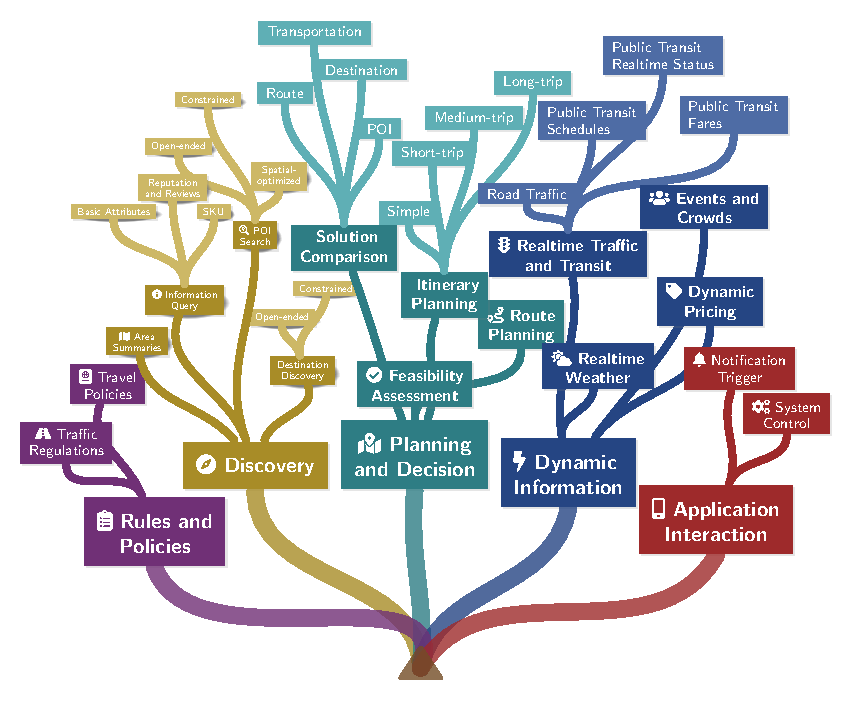
\includegraphics[width=1\textwidth]{resources/intent-tree.pdf}
  \caption{A visual taxonomy of our intent classification system. The hierarchical structure is organized into five primary categories: Rules and Policies, Discovery, Planning and Decision, Dynamic Information, and Application Interaction. The taxonomy further branches into 16 second-level categories and terminates in 30 fine-grained leaf nodes, capturing the multi-faceted complexity of real-world user queries in navigation and travel scenarios.}
  % \vspace{-20pt}  % ⭐ 增大负值，减少下方空白
  \label{fig:intent_taxonomy}
\end{figure}

{\textbf{Stage 1: Seed Initialization.}} We manually curate a small, high-variance set of $n$ seed prompts ($\mathcal{D}_{seed} \in \mathcal{D}_{pool}$) to represent the core diversity of the domain. Experts annotate these seeds with open-ended tags to capture abstract intent features. Each query is mapped into a tuple as:

$$\mathcal{S}_i = \langle q_i, \mathcal{T}_i \rangle, \text{ s.t. } \mathcal{T}_i = \{t_{i,1}, t_{i,2}, \dots, t_{i,k}\},$$

where $\mathcal{T}_i$ denotes the $k$ orthogonal or complementary intent nodes covered by instruction $q_i$.

{\textbf{Stage 2: LLM-Driven Category Induction.}} Using the annotated seeds, we prompt an LLM to induce orthogonal Level-1 categories, ensuring granular alignment across the domain.

{\textbf{Stage 3: Iterative Refinement Loop.}} To prevent hallucinations, we implement a strict check-update cycle. The LLM re-annotates the $\mathcal{D}_{seed}$ using the generated categories; human experts review these annotations to identify ambiguity or coverage gaps, feeding feedback back to the LLM for taxonomy refinement, executing a ``Tag-Feedback-Correction" cycle across several iterations:

$$\mathcal{T}^{(k+1)} = \text{Refine}\left( \text{Annotate}(\mathcal{D}_{seed}, \mathcal{T}^{(k)}), \text{Human\_Feedback} \right)$$

During this process, human experts identify ambiguity or coverage gaps in the LLM-generated categories, feeding critical insights back for taxonomy adjustment. The process terminates when $\mathcal{T}^{(k+1)} \approx \mathcal{T}^{(k)}$, signifying that the system has converged into a stable benchmark taxonomy $\mathcal{T}^*$.

{\textbf{Stage 4: Dynamic Taxonomy Expansion.}} To capture long-tail intents beyond the initial seeds, we enforce an ``Other" category at each node. By labeling a massive scale of raw logs and analyzing samples falling into the ``Other" category, we discover and merge emerging categories, allowing the taxonomy to evolve dynamically.


This mechanism transforms the taxonomy from a static tree into an evolving system capable of adapting to the open-world distribution of user queries. The resulting finalized Intent Taxonomy is visualized in Figure~\ref{fig:intent_taxonomy}.

\subsubsection{Annotation and Data Curation}


Building upon this stabilized and mutually orthogonal taxonomy, we deployed a high-capacity teacher LLM to execute large-scale intent classification on the structured log data. The specific prompt template used for this annotation is detailed in Appendix \ref{app:intent_classification_prompt}. To ensure the training data achieves both high information density and minimal redundancy, we implemented a rigorous two-phase process:

\textbf{Precise Multi-Dimensional Annotation.} We treat intent understanding as a multi-label classification task. Each user instruction is mapped to a composite label vector $\mathcal{V} = \langle I_{primary}, I_{secondary}, \mathcal{C}_{constraints} \rangle$.

\begin{itemize}
\item $I_{primary}$ and $I_{secondary}$ represent the leaf nodes in our fine-grained Intent Taxonomy.

\item $\mathcal{C}_{constraints}$ captures specific auxiliary dimensions (e.g., \textit{spatial\_range}, \textit{time\_budget}, \textit{vehicle\_type}).

\end{itemize}

This granular tagging captures the semantic nuance of complex queries, distinguishing between simple keyword searches and multi-constraint planning tasks.

\textbf{Controlled Sampling via Funnel Filtering.} 
Based on the annotation results, we applied a three-stage \textbf{Funnel Filtering Strategy} to construct the final curated dataset. This pipeline systematically eliminates redundancy at lexical, semantic, and geometric levels:
\begin{itemize}
    \item \textbf{Lexical Redundancy Elimination:} We applied global Locality-Sensitive Hashing \textbf{at corpus level} to efficiently remove near-duplicate strings and literal repetitions (``garbage data'') across all data, significantly reducing the initial volume.
    \item \textbf{Semantic Redundancy Elimination:} To ensure high intra-class variance, we partitioned the dataset into buckets based on the $\langle I_{primary}, I_{secondary} \rangle$ tuple. Within each bucket, we performed embedding-based similarity search to prune semantically redundant samples—defined as distinct phrasings that reside within a predefined distance threshold in the latent space. To handle the scale of our dataset, we integrated Faiss to accelerate this process; this transitioned the computational complexity from a quadratic $O(N^2)$ brute-force pairwise comparison to a more scalable sub-linear or near-linear search complexity, significantly reducing the preprocessing overhead.
    % Within each bucket, we utilized embedding-based similarity search to identify and prune semantically redundant samples (e.g., removing distinct phrasings that map to identical semantic vectors), ensuring high variance within each intent category.
    \item \textbf{Geometric Redundancy Elimination:} From the remaining pool, we employed the K-Center-Greedy algorithm to select the most representative samples. By maximizing the minimum distance between selected data points in the embedding space, this step preserves long-tail and corner-case queries that are critical for robust agent performance.
\end{itemize}

\begin{figure}[h]
  \centering
  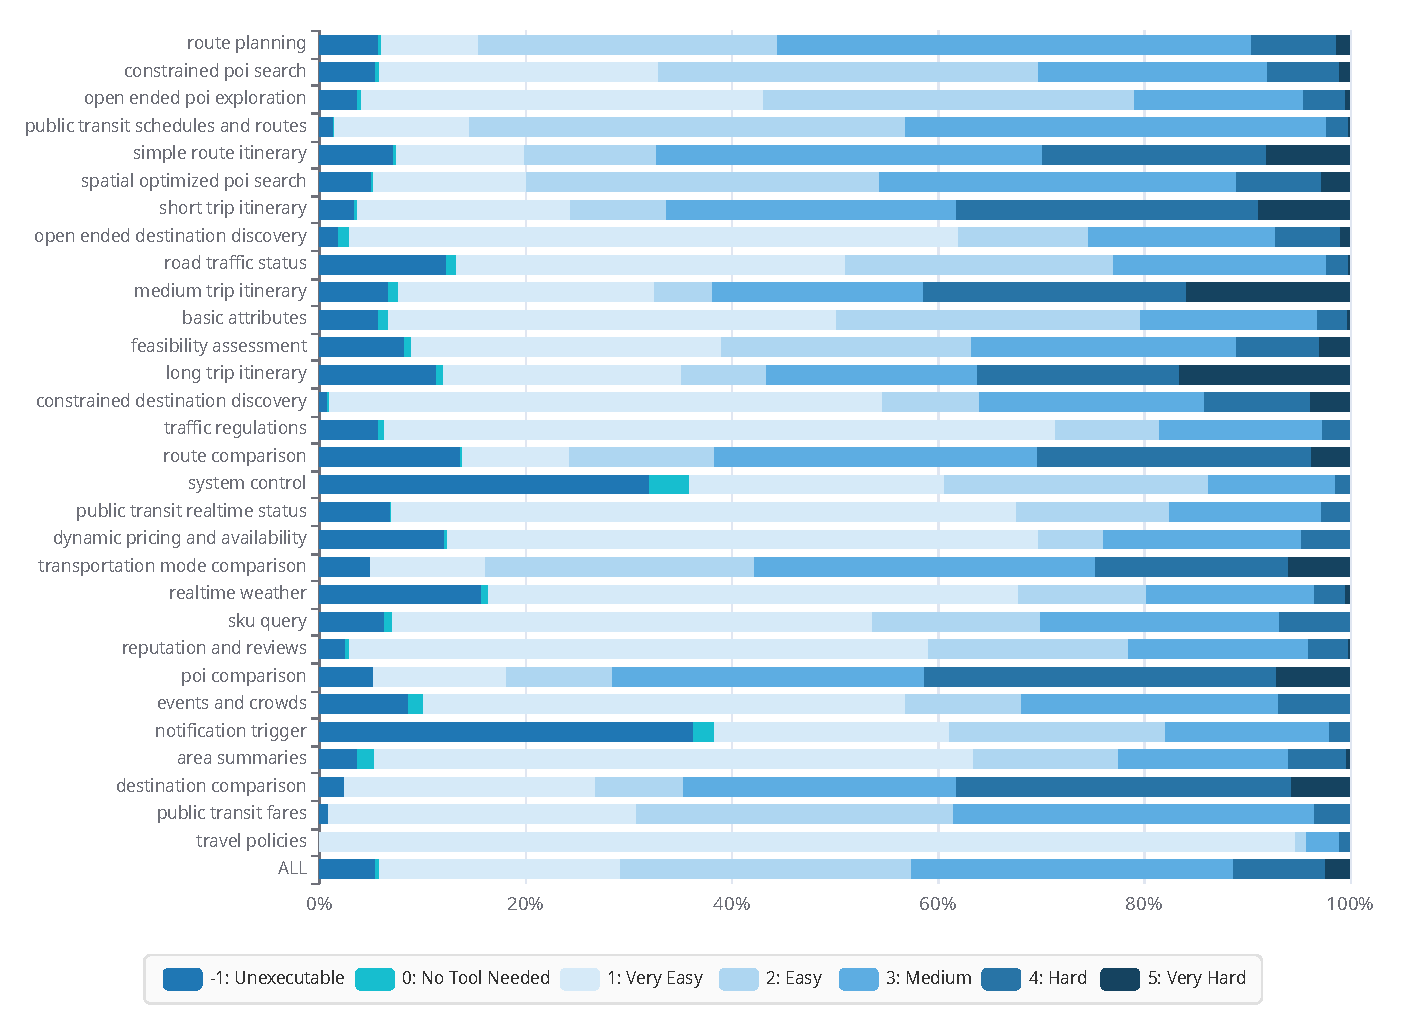
\includegraphics[width=0.98\textwidth]{resources/difficulty-distribution.pdf}
  \caption{\textbf{Fine-grained Difficulty Distribution across 30 Geospatial Domains.} The visualization reveals the distinct complexity profiles of different tasks. While atomic queries (e.g., \textit{basic attributes}) cluster in low-difficulty regions (Score 1-2), composite tasks (e.g., \textit{long trip itinerary}) exhibit a significant proportion of high-complexity reasoning (Score 4-5). The visible segments of Score -1 and 0 (denoted as \textbf{Ext.1}) across domains like \textit{System Control} highlight our active sampling of boundary cases for hallucination mitigation.}
  \label{fig:prefilter-difficulty}
\end{figure}

\subsubsection{Difficulty and Diversity}
Real-world geospatial tasks vary significantly in cognitive load. To ensure the \model demonstrates robustness across this spectrum, we rigorously stratified our training data. Beyond mere coverage, the primary objective of this stratification is to enable Difficulty-based Curriculum Learning. In RL, a static data distribution often leads to training inefficiency: early-stage models facing excessively hard tasks yield zero rewards (vanishing gradients), while late-stage models facing trivial tasks yield constant perfect rewards (lack of variance). To address this, we employed an \textbf{Execution-Simulation Scoring Mechanism} to label data complexity, allowing us to dynamically align training data with model proficiency. This mechanism evaluates difficulty across three orthogonal dimensions:

\begin{itemize}
\item \textbf{Cognitive Load in Tool Selection:} Measures the ambiguity of intent mapping. It spans from \textit{Explicit Mapping} (Score 1-2, e.g., ``Navigates to X'') to \textit{Implicit Reasoning} (Score 4-5, e.g., ``Find a quiet place to read within a 20-minute drive,'' requiring abstract intent decomposition). 
\item \textbf{Execution Chain Depth:} Quantifies the logical complexity of the solution path, tracking the number and type of tool invocations and dependency depth (e.g., sequential vs. parallel execution). 
\item \textbf{Constraint Complexity:} Assesses the density of constraints (spatial, temporal, and preferential) that the agent must jointly optimize. 
\end{itemize}

To operationalize this mechanism at scale, we utilize a strong teacher LLM as an automated evaluator. This evaluator analyzes the structured user logs, assessing them against the three critical competencies to assign a scalar difficulty score $r \in \{-1, 0, 1, ..., 5\}$ to each sample. The specific prompt template used for this evaluation is detailed in Appendix \ref{app:difficulty_scoring_prompt}.

To validate the efficacy of this scoring mechanism, we visualize the distribution of annotated samples across 30 domains in Figure \ref{fig:prefilter-difficulty}. The distribution aligns intuitively with task semantics, providing strong support for our curriculum strategy:
\begin{itemize}\item \textbf{Spectrum Coverage for Curriculum Learning:} As shown in the ``ALL" bar at the bottom of Figure \ref{fig:prefilter-difficulty}, the aggregated dataset achieves a balanced stratification. This allows us to construct training batches that progressively shift from ``Atomic Operations" (Score 1-2) to ``Complex Reasoning" (Score 4-5) throughout the training lifecycle, preventing the reward collapse issues mentioned above.\item \textbf{Domain-Specific Complexity Profiles:} The scorer correctly identifies the inherent hardness of different intents. For instance, \textit{Long-trip Itinerary} is dominated by Score 4-5 samples (dark blue segments), reflecting its need for multi-constraint optimization. In contrast, \textit{Traffic Regulations} consists primarily of Score 1-2 samples, confirming the scorer's ability to distinguish between retrieval and reasoning tasks.
\end{itemize}

By curating batches based on these scores, we ensure the \model receives a consistent gradient signal throughout its training lifecycle. Furthermore, we place special emphasis on boundary conditions to enhance reliability:




\paragraph{Irrelevance and Hallucination Mitigation (Score -1/0).} A critical failure mode in agents is the tendency to hallucinate actions for unsolvable queries. To mitigate this, it is critical to train models to explicitly reject unanswerable queries or seek alternative solutions when desired tools are unavailable.

To achieve this, we constructed a dedicated \textbf{Irrelevance Dataset} (denoted as \textbf{Ext.1} in Figure \ref{fig:prefilter-difficulty}). By training on these negative samples, the \model learns to recognize the boundaries of its toolset, significantly reducing hallucination rates in open-world deployment.